\documentclass[a4paper,12pt]{report}
\usepackage[utf8]{inputenc}
\usepackage[francais]{babel}
\usepackage{fancyhdr}
\usepackage{graphicx}
\usepackage{tikz}
\usetikzlibrary{calc}
\usepackage{listings}
\usepackage{xcolor}
\definecolor{grey}{rgb}{0.9,0.9,0.9}
\usepackage{titlesec}
\usepackage{verbatim}
\usepackage{listings}
\usepackage{textcomp}
\usepackage{hyperref}
\usepackage{ amssymb }


\frenchbsetup{StandardLists=true}
\newcommand{\marge}{18mm}
\usepackage[left=\marge,right=\marge,top=\marge,bottom=\marge]{geometry}
\pagestyle{fancy}
\setlength{\headheight}{14pt}
\chead{
  \textbf{Binôme :} Douaille Erwan \& François Rémy
  \hspace{2em}
  \textbf{Groupe :} M1 Info RDF}
\renewcommand{\headrulewidth}{1pt}
\linespread{1}
\setlength{\columnseprule}{0.2pt}





\begin{document}


\makeatletter
\begin{titlepage}
\centering
\vspace{-10em}
{\LARGE \textbf{\textsc{Rapport de Projet RVI}}}\\
\vspace{3em}

\includegraphics[scale=0.6]{image/thalassa.png}\\
\vspace{3em}
{\LARGE \textsc{Projet Thalassa: simulation de plongée sous-marine}}\\

\vspace{8em}
Par\\
\vspace{1em}
{\LARGE \@author}\\

\vspace{2em}



\begin{tikzpicture}[remember picture,overlay]

\node [below left,xshift=-1cm, yshift=4cm] at (current page.south east){
\includegraphics[scale=0.6]{image/ustl1.png}};

\end{tikzpicture}
\end{titlepage}
\makeatother

\sloppy

\setcounter{page}{1} 
\newpage

\section*{Introduction}

Dans ce TP nous allons comparer deux méthodes de reconnaissance des formes. L'algorithme de Fourier et l'algorithme des cordes. Nous allons comprendre quels sont leurs intérêts et leurs limites pour faire de la reconnaissance de formes.

\section*{Code R}

\subsection*{Comment sont codés les points du contour dans la variable cont?}

La variable cont contient un vecteur d'équation x+y*i. Chaque équation correspondant aux coordonnées d'un point.

\subsection*{Quel est l'intérêt du dernier argument de la méthode plot?}

Le dernier argument nous permet d'obtenir un intervalle définit par les min, max des nombres imaginaires. Cet intervalle définit les limites des coordonnées y.

\begin{figure}[!ht]
	\center
	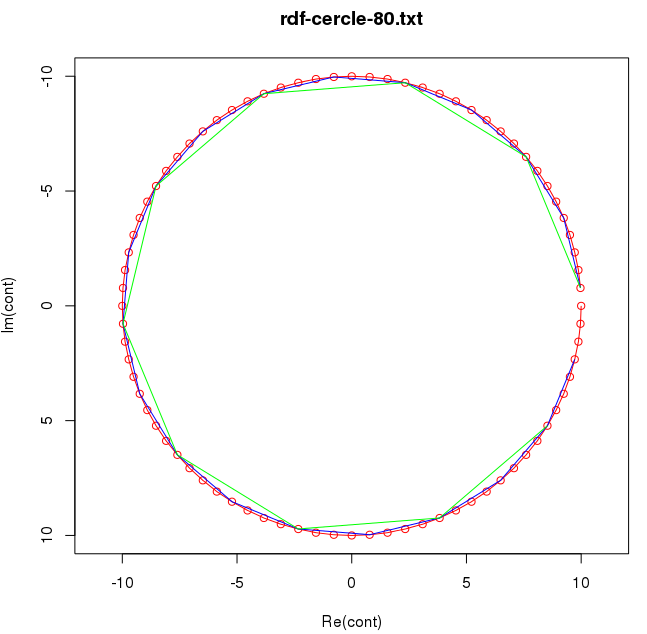
\includegraphics[scale=0.5]{image/contours.png}
\end{figure}

Cette partie nous a apprit à créer des contours à utiliser plot et à savoir comment sont codés les points. 

\newpage 









\section*{Descripteur de Fourier}

Les descripteurs de Fourier nous permettent de compacter les données. 


\begin{figure}[!ht]
	\hbox{ 
     	\hspace*{1cm}
		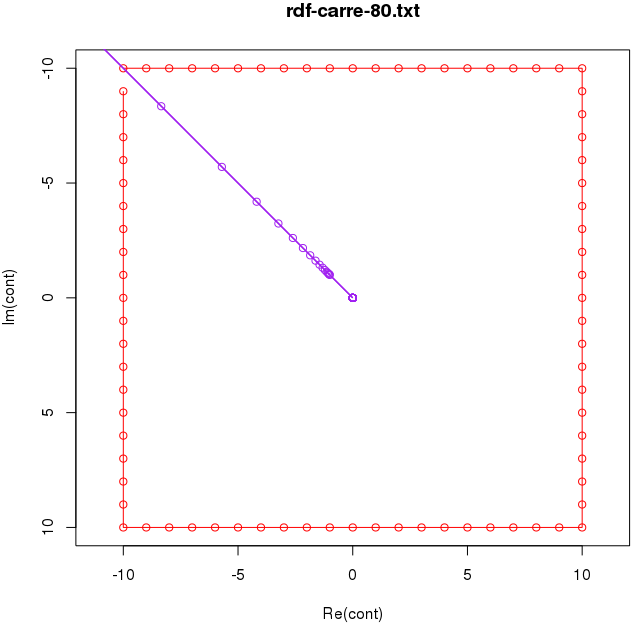
\includegraphics[scale=0.3]{image/fourier1.png}
     	\hspace*{1cm}
		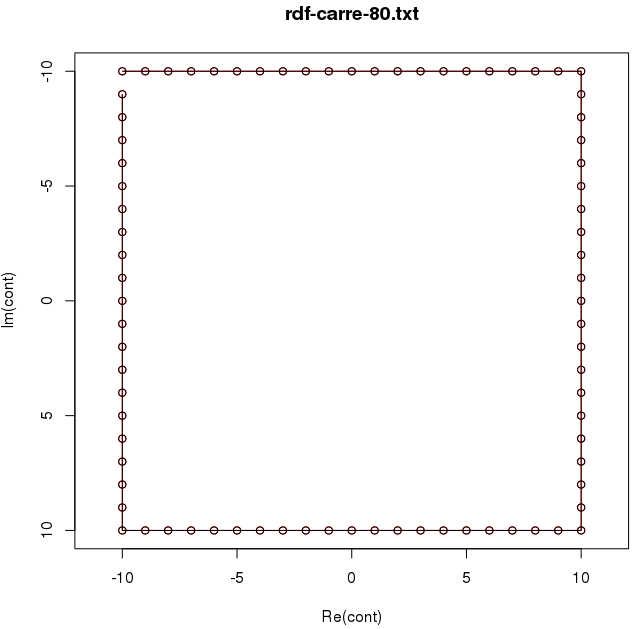
\includegraphics[scale=0.3]{image/fourier2.png}
	}
\end{figure}

Içi on peut voir sur l'image de gauche la description de Fourier (courbe violette) et sur l'image de droite l'inverse de cette desciprition de Fourier (carré noir recouvrant le carré rouge). La description de Fourier représente le carré sous forme compacte et en testant l'inverse de cette description de Fourier on retrouve bien le carré original (superposition du carré noir et le carré rouge).

Le descripteur de Fourier Z0 correspond au barycentre. C'est le premier élément de notre tableau. Il à pour valeur 0+0i car il est centré à l'origine

\begin{figure}[!ht]
	\hbox{ 
     	\hspace*{1cm}
		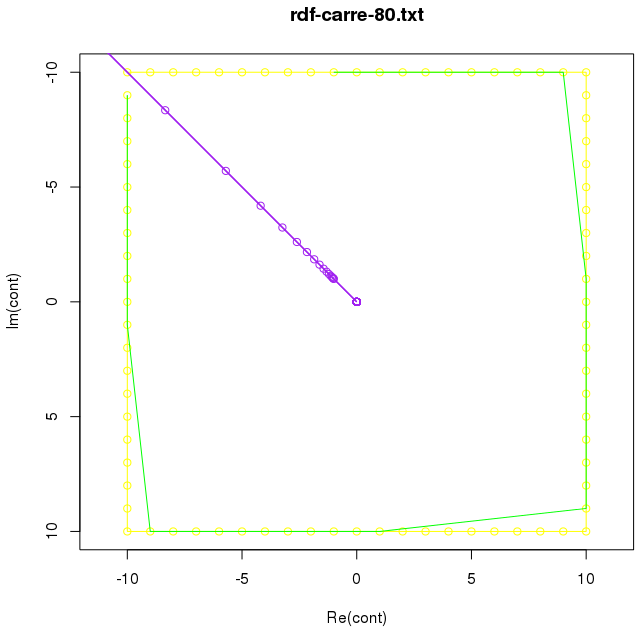
\includegraphics[scale=0.3]{image/fourier3.png}
     	\hspace*{1cm}
		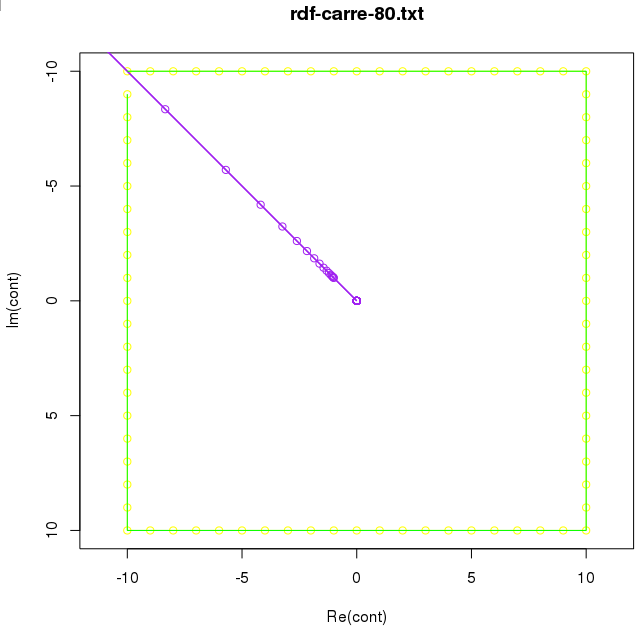
\includegraphics[scale=0.3]{image/fourier4.png}
	}
\end{figure}

Grâce à la fonction rdfAnnuleDescFourier on réduit le nombre de points. On peut constater que même avec un ratio de 0.1 (image de gauche) le carré de base est représenté, avec quelques erreurs. L'image de droite avec un ratio de 0.8 respecte parfaitement le carré original.

\newpage




\section*{Réduction d'une chaîne de contour}

\begin{figure}[!ht]
	\center
	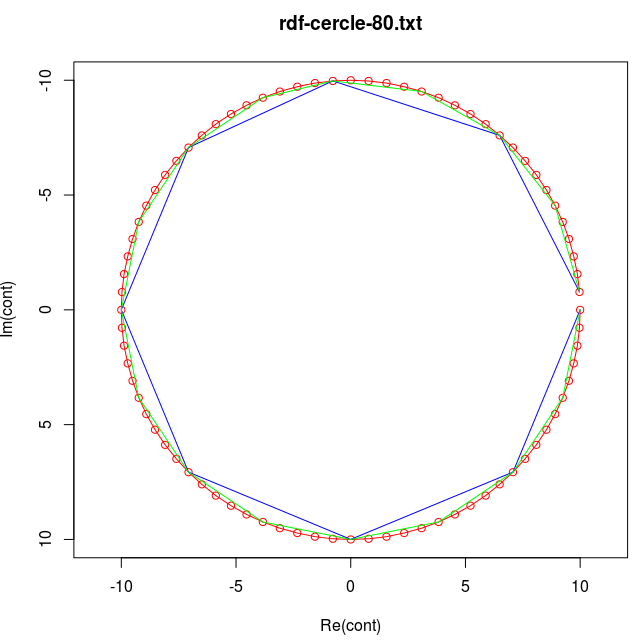
\includegraphics[scale=0.5]{image/fourier5.png}
\end{figure}


Sur la figure ci-dessus, on peut voir les différences entre la courbe initial en rouge, la version dmax=0.5 en vert et la version dmax=1 en bleu.

On peut donc dire que ca permet également d'approcher la forme du cercle. Plus on met une distance petite, plus ce sera fidèle au cercle initial.

\newpage






\section*{Comparaison des deux approches}

\begin{figure}[!ht]
	\hbox{ 
     	\hspace*{1cm}
		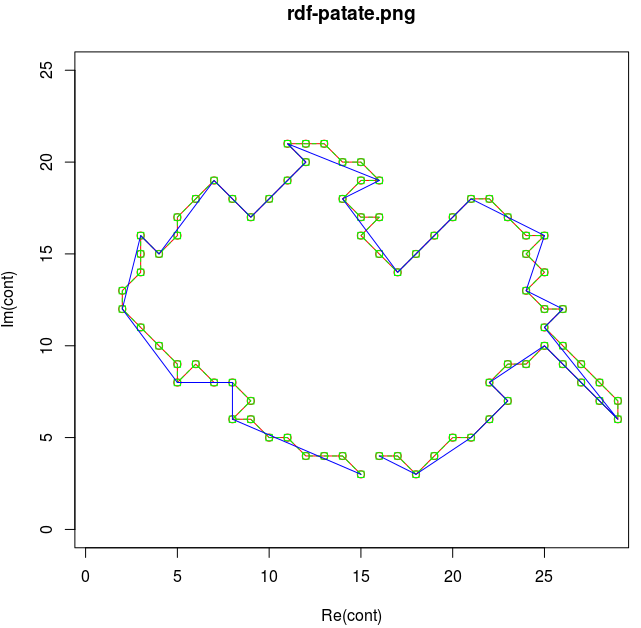
\includegraphics[scale=0.3]{image/fourier6.png}
     	\hspace*{1cm}
		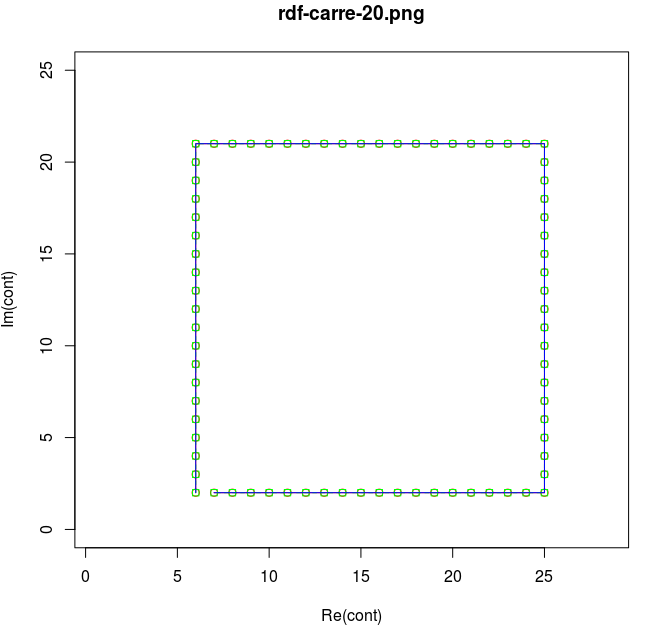
\includegraphics[scale=0.3]{image/fourier7.png}
	}
	\hbox{ 
     	\hspace*{1cm}
		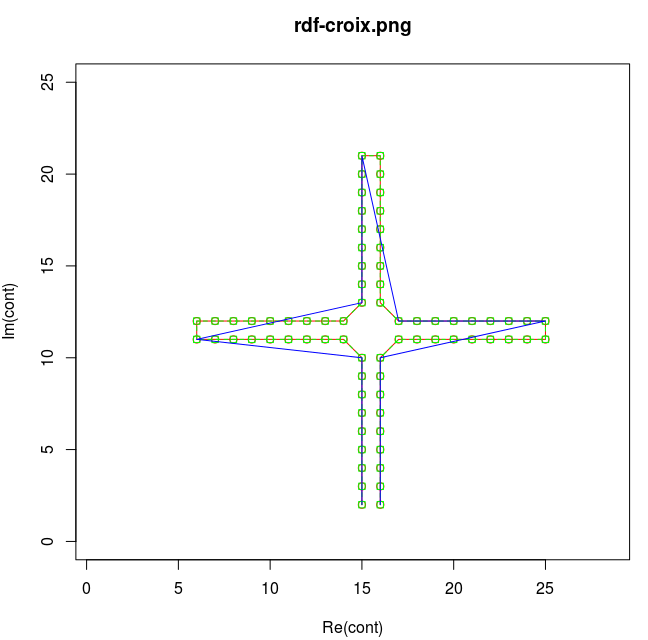
\includegraphics[scale=0.3]{image/fourier8.png}
     	\hspace*{1cm}
		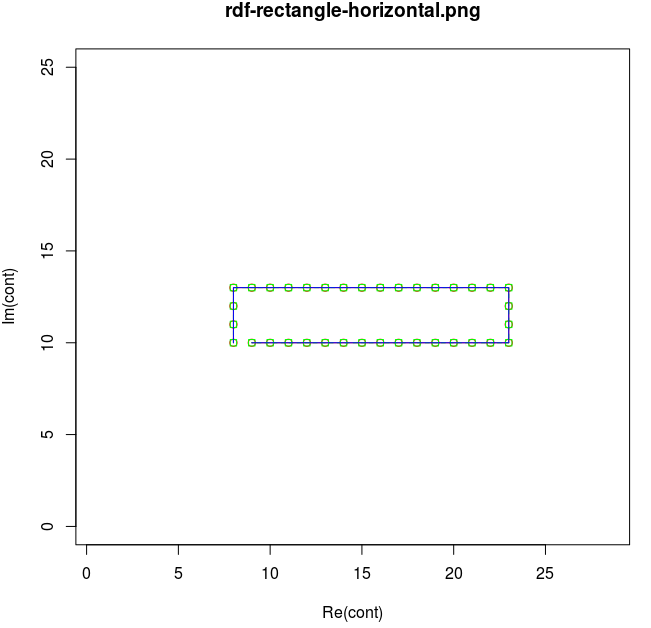
\includegraphics[scale=0.3]{image/fourier9.png}
	}
\end{figure}

Dans la comparaison on remarque nettement que l'algorithme de Fourier (en vert) retourne une forme fidèle à l'original (en rouge) que la forme soit complexe ou non. Concernant l'algorithme des cordes (en bleu) on voit clairement ses limites dans les formes complexes la patate ou la croix. L'algorithme des cordes est pourtant très précis sur les formes géométriques simples.


\section*{Conclusion}

Pour conclure, on voit clairement sur les figures que l'algorithme de Fourier est beaucoup plus précis, notamment sur le patatoide. On peut donc dire que dans le cadre d'une reconnaissance de formes sur des formes complexes ou des images réels l'algorithme de Fourier sera à utiliser, tandis que l'algorithme des cordes fera parfaitement son travail sur de la reconnaissance de formes géométriques simples du style carré, triangle.


\end{document}
